\documentclass{beamer}

%\usetheme{Copenhagen}
%\usetheme{AnnArbor}
\usetheme%[outer/progressbar=foot,outer/numbering=none]
{metropolis}

\usepackage{graphicx}
\usepackage{graphicx} %Loading the package
\graphicspath{{images/}} %Setting the graphicspath
%\usepackage{xcolor}


\usepackage{pgfplots}

%draw multipage tables
\usepackage{longtable}
%draw horizontal  rules in tables
\usepackage{booktabs}
%enable multipage table header repeat
\usepackage{xtab}
%enable set width columns in xtabular
\usepackage{array}
%enable caption in xtabular tables
\usepackage{caption}
%enable \Verb command inside tables
\usepackage{fvextra}
%trim and clip box material
\usepackage{trimclip}
%build gantt chart
\usepackage{styles/gantt}
\newcommand{\defcolor}{red}
%\usepackage{pgfgantt}



%output code listings : 3 packages
\usepackage{listings}
\usepackage[T1]{fontenc}
\usepackage{lmodern}
%creates a box named \codebox to store code listings
\newsavebox{\codebox}% For storing  code listings

%draw figures and gannt charts
\usepackage{tikz}


%print license Disclaimer using \ccbysa command
\usepackage[scale=2]{ccicons}

%create \themename command to point to metropolis
\usepackage{xspace}
\newcommand{\themename}{\textbf{\textsc{metropolis}}\xspace}


%\definecolor{Purple}{HTML}{911146}
%\setbeamercolor{frametitle}{bg=Purple}
%\definecolor{Alternate}{HTML}{3366cc}
%\setbeamercolor{frametitle}{bg=Alternate}

%change fonts to other alternatives
%\usepackage[sfdefault]{sourcesanspro}
%recommended for metropolis theme
\usepackage[sfdefault]{FiraSans}


\usepackage{adjustbox}
%---------------

\title{Creating Polished Presentations}
\date{West New York, \today.}
\author{Valerii Klymchuk \\ www.voklymchuk.com}
\institute{Centre for Modern Templates}


\begin{document}
\maketitle



\begin{frame}{Outline}
	\tableofcontents
\end{frame}

\begin{frame}[standout]
	Thanks for your attention.
	Pay attention here...
\end{frame}

 %---------------
\section{Introduction} 

\begin{frame}
	This is going to be a normal paragraph in our introduction.
	
	
		Some intro stuff
		\begin{block}{Observation}
			This is a very important piece of information.
		\end{block}
		Some other stuff ...


\end{frame}





\begin{frame}{Blocks}
	Three different block environments are pre-defined and may be styled with an
	optional background color.
	
	\begin{columns}[T,onlytextwidth]
		\column{0.5\textwidth}
		\begin{block}{Default}
			Block content.
		\end{block}
		
		\begin{alertblock}{Alert}
			Block content.
		\end{alertblock}
		
		\begin{exampleblock}{Example}
			Block content.
		\end{exampleblock}
		
		\column{0.5\textwidth}
		
		\metroset{block=fill}
		
		\begin{block}{Default}
			Block content.
		\end{block}
		
		\begin{alertblock}{Alert}
			Block content.
		\end{alertblock}
		
		\begin{exampleblock}{Example}
			Block content.
		\end{exampleblock}
		
	\end{columns}
\end{frame}




\section{Tables, figures and subfiles}\label{sec:background}

\subsection{Tables and Figures}

\begin{frame}
To insert a figure, you can use the TeXnicecenter menus. 
\begin{figure}
	\centering
	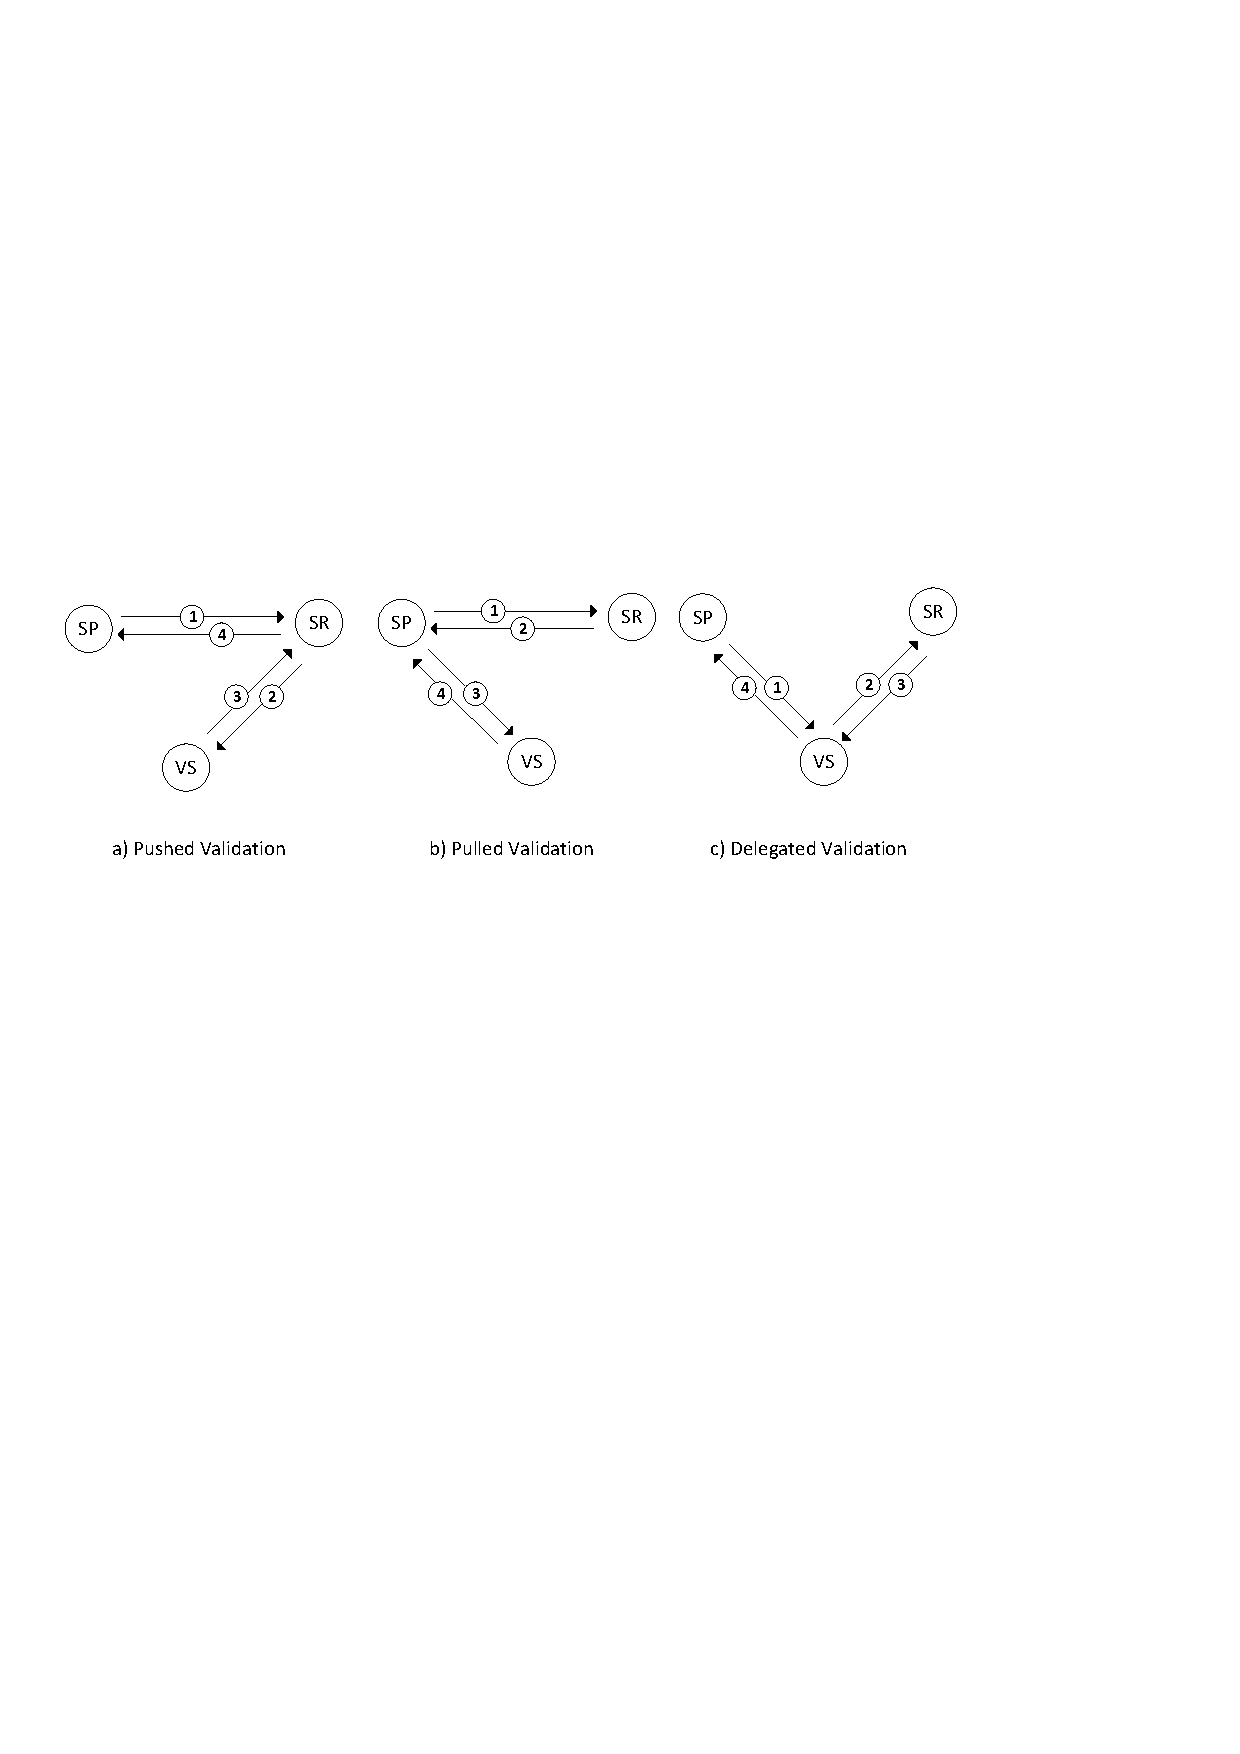
\includegraphics[width=1.00\linewidth]{att-models-base.pdf}
	\caption{My First Figure}
	\label{fig:att-models-base}
\end{figure}

\end{frame}






\begin{frame}[fragile,allowframebreaks]{Multipage Xtabular table}
\begin{table}
	\tablecaption
	{
		Sample multipage table with repeating header 
	}
	\label{tab:MyFirstTable}
	\tablefirsthead{
		\toprule  & \bf document class  &\bf bibliography style &   \\ \midrule
	}
	\tablehead{
		\\
		\multicolumn{4}{c}{\text{\tablename~\thetable{}  continued }} \\
		\midrule &\bf document class &\bf bibliography style &  \\ \midrule
	}

	\begin{xtabular}{
			p{0.25\linewidth}
			p{0.27\linewidth}
			p{0.17\linewidth}
			m{0.15\linewidth}
		}
		Institute of Electrical and Electronics Engineers &\Verb|IEEEtran| & \Verb|IEEEtran|& \raisebox{-0.5\totalheight}{
\includegraphics[width=1\linewidth]{ieee.png}}\\ \midrule
		Association for Computing Machinery & \Verb|sig-alternate|  & \Verb|plain| & \raisebox{-0.5\totalheight}{
\includegraphics[width=1\linewidth]{acm.jpeg}}   \\ \midrule
		Lecture Notes in Computer Science& \Verb|llncs|& \Verb|splncs|& \raisebox{-0.5\totalheight}{
\includegraphics[width=1\linewidth]{llncs.png}}  \\ \midrule
		General & \Verb|article|  & \Verb|plain|  &  \\ 
		
		\bottomrule
	\end{xtabular}
\end{table}
\end{frame}




\begin{frame}
\subsection{Cross-references} 
Some text here that wants to refer to Table~\ref{tab:MyFirstTable}. You can also refer to the Figure~\ref{fig:att-models-base}. When you want to refer to a previous section, you can use the \Verb|\ref| command again. Section~\ref{sec:background}.%Section~\ref{sec:drilled-down}. 

\subsection{Sub section through input command}
This comes from a separate file. Notice that we have this subsection included in the Navigator.  

\end{frame}






	









\section{Drawing pictures}\label{sec:background}


\begin{frame}{Tikspictures}
\begin{figure}
	%\resizebox{\linewidth}{!}{
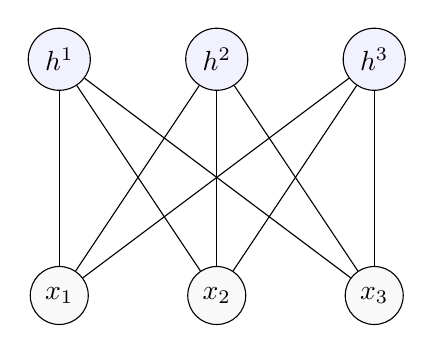
\begin{tikzpicture}	
\tikzset{
	hcirc/.style={
		draw, circle, fill=blue!5
	},
	xcirc/.style={
		hcirc, fill=gray!5
	}
}

\foreach \i in {1, ..., 3}{
	\node [hcirc] (h\i) at (\i*2,3) {$h^\i$};
}

\foreach \i in {1, ..., 3}{
	\node [xcirc] (x\i) at (\i*2,0) {$x_\i$};
}

\foreach \i in {1, ..., 3}{
	\foreach \v in {1, ..., 3}{
		\path (h\i) edge [draw] (x\v);
	}
}
\end{tikzpicture}
%}	
\caption{M1} \label{fig:M1}
\end{figure}
\end{frame}





\section{Code Listings}

\lstset{language=[LaTeX]tex}
\lstset{caption=Some \LaTeX Code}
\begin{lrbox}{\codebox}
	\begin{lstlisting}[frame=single]{}
	\begin{frame}
	\titlepage
	\end{frame}
	\end{lstlisting}
\end{lrbox}
\begin{frame}{\LaTeX Code}
	\usebox{\codebox}
\end{frame}



\lstset{language=c++}
\lstset{caption=Some C++ Code}
\begin{lrbox}{\codebox}
	\begin{lstlisting}[frame=single, basicstyle=\ttfamily]{}
	for(i = 0; i < 10; i++){
	// increment the pointer
	*p++ = i;
	}
	\end{lstlisting}
\end{lrbox}
\begin{frame}{Code}
	\usebox{\codebox}
\end{frame}

\section{Gantt charts}

\begin{frame}{Gant charts}
	\begin{table}
		\centering
		\resizebox{\linewidth}{!}
		{
			\begin{gantt}[drawledgerline=true, xunitlength=\linewidth/25]{11}{24}
				% vertical, horizontal 'boxes'
				\begin{ganttitle}
					\numtitle{2012}{3}{2012}{10}
					% start, label, width 
					\numtitle{2013}{1}{2013}{12}
					\numtitle{2014}{1}{2014}{2}
				\end{ganttitle}
				\begin{ganttitle}
					\numtitle{3}{1}{12}{1}
					% start, skip, end, width 
					\numtitle{1}{1}{12}{1}
					\numtitle{1}{1}{2}{1}
				\end{ganttitle}
				\ganttmilestone{Proposal Defense}{0} % Label, position
				%=======================================
				\ganttgroup{Background Study}{0}{6} % start, width 
				\ganttbar[color=\defcolor]{Android Security}{0}{3}
				\ganttbarcon[color=\defcolor]{Code Analysis}{3}{2}
				\ganttbarcon[color=\defcolor]{Policy Mechanisms}{5}{1}
				\ganttmilestonecon{Literature Review Complete}{6}
				% notice the 'con' at the end -- for continue 
				%=======================================
				\ganttbarcon[color=\defcolor]{
					\textbf{Formal Specification} % can format labels!
				}{6}{6}
				\ganttmilestonecon{Spec Document}{12}
				%=======================================
				\ganttbar[color=blue]{Thesis and Paper Writing}{0}{24}
			\end{gantt}

		}	
		\caption{My First Gantt}\label{fig:gantt-1}
		
	\end{table}
\end{frame}


%\begin{frame}
%	\begin{figure}[ftbp]
%		\begin{center}
%			
%			\begin{ganttchart}[y unit title=0.4cm,
%				y unit chart=0.5cm,
%				vgrid,hgrid, 
%				title label anchor/.style={below=-1.6ex},
%				title left shift=.05,
%				title right shift=-.05,
%				title height=1,
%				bar/.style={fill=gray!50},
%				incomplete/.style={fill=white},
%				progress label text={},
%				bar height=0.7,
%				group right shift=0,
%				group top shift=.6,
%				group height=.3,
%				group peaks height={}{}{.2}]{1}{24}
%				%labels
%				\gantttitle{Week}{24} \\
%				\gantttitle{Monday}{4} 
%				\gantttitle{Tuesday}{4} 
%				\gantttitle{Wednesday}{4} 
%				\gantttitle{Thursday}{4} 
%				\gantttitle{Friday}{4} 
%				\gantttitle{Saturday}{4} \\
%				%tasks
%				\ganttbar{first task}{1}{2} \\
%				\ganttbar{task 2}{3}{8} \\
%				\ganttbar{task 3}{9}{10} \\
%				\ganttbar{task 4}{11}{15} \\
%				\ganttbar[progress=33]{task 5}{20}{22} \\
%				\ganttbar{task 6}{18}{19} \\
%				\ganttbar{task 7}{16}{18} \\
%				\ganttbar[progress=0]{task 8}{21}{24}
%				
%				%relations 
%				\ganttlink{elem0}{elem1} 
%				\ganttlink{elem0}{elem3} 
%				\ganttlink{elem1}{elem2} 
%				\ganttlink{elem3}{elem4} 
%				\ganttlink{elem1}{elem5} 
%				\ganttlink{elem3}{elem5} 
%				\ganttlink{elem2}{elem6} 
%				\ganttlink{elem3}{elem6} 
%				\ganttlink{elem5}{elem7} 
%			\end{ganttchart}
%		\end{center}
%		\caption{Gantt Chart}
%	\end{figure}
%\end{frame}



%\begin{frame}{Appearing lines}
%	Putting some content in ...
%	
%	\pause 
%	Second Line ...
%	
%	\pause
%	Third line ..
%\end{frame}




\begin{frame}{Line plots}
	\begin{figure}
		\begin{tikzpicture}
		\begin{axis}[
		mlineplot,
		width=0.9\textwidth,
		height=6cm,
		]
		
		\addplot {sin(deg(x))};
		\addplot+[samples=100] {sin(deg(2*x))};
		
		\end{axis}
		\end{tikzpicture}
	\end{figure}
\end{frame}





\begin{frame}{Bar charts}
	\begin{figure}
		\begin{tikzpicture}
		\begin{axis}[
		mbarplot,
		xlabel={Foo},
		ylabel={Bar},
		width=0.9\textwidth,
		height=6cm,
		]
		
		\addplot plot coordinates {(1, 20) (2, 25) (3, 22.4) (4, 12.4)};
		\addplot plot coordinates {(1, 18) (2, 24) (3, 23.5) (4, 13.2)};
		\addplot plot coordinates {(1, 10) (2, 19) (3, 25) (4, 15.2)};
		
		\legend{lorem, ipsum, dolor}
		
		\end{axis}
		\end{tikzpicture}
	\end{figure}
\end{frame}






{%
	\setbeamertemplate{frame footer}{My custom footer}
	\begin{frame}[fragile]{Frame footer}
		\themename defines a custom beamer template to add a text to the footer. It can be set via
		\begin{verbatim}\setbeamertemplate{frame footer}{My custom footer}\end{verbatim}
	\end{frame}
}

\begin{frame}{References}
	Some references to showcase~\cite{knuth92,ConcreteMath,Simpson,Er01,greenwade93}
\end{frame}

\section{Conclusion}

\begin{frame}{Summary}
	
	Get the source of this theme and the demo presentation from
	
	\begin{center}\url{github.com/voklymchuk/mtheme}\end{center}
	
	The theme \emph{itself} is licensed under a
	\href{http://creativecommons.org/licenses/by-sa/4.0/}{Creative Commons
		Attribution-ShareAlike 4.0 International License}.
	
	\begin{center}\ccbysa\end{center}
	
\end{frame}

\begin{frame}[standout]
	Questions?
\end{frame}

\appendix

\begin{frame}[fragile]{Backup slides}
	Sometimes, it is useful to add slides at the end of your presentation to
	refer to during audience questions.
	
	The best way to do this is to include the \verb|appendixnumberbeamer|
	package in your preamble and call \verb|\appendix| before your backup slides.
	
	\themename will automatically turn off slide numbering and progress bars for
	slides in the appendix.
\end{frame}




%\section{Background} %--------------


%\begin{frame}[fragile, allowframebreaks]{Using longtable }
%\begin{longtable}[ht]{
%		p{0.25\linewidth}
%		p{0.27\linewidth}
%		p{0.17\linewidth}
%		m{0.15\linewidth}
%	} % <-- Replaces \begin{table}, alignment must be specified here (no more tabular)
%	\caption{Multipage table without repeating header}
%	\label{tab:table1}\\
%	\toprule
%	& \bf document class& \bf bibliography style & \\
%	\midrule
%\endfirsthead 
%
%\toprule
%& \bf document class& \bf bibliography style & \\
%\midrule
%
%\endhead
%
%	
%	Institute of Electrical and Electronics Engineers & \verb|IEEEtran| 											& \verb|IEEEtran| & \raisebox{-0.5\totalheight}{
\includegraphics[width=1\linewidth]{ieee.png}}   \\ \midrule
%	Association for Computing Machinery               & \verb|sig-alternate|                                       & \verb|plain|                    & \raisebox{-0.5\totalheight}{
\includegraphics[width=1\linewidth]{acm.jpeg}}   \\ \midrule
%	Lecture Notes in Computer Science                 & \verb|llncs|                                            & \verb|splncs|                 & \raisebox{-0.5\totalheight}{
\includegraphics[width=1\linewidth]{llncs.png}}  \\ \midrule
%	IEEE Computer Society                             & {\verb|[twocolumn]| \verb|{article}|  \verb|\usepackage|  \verb|{latex8}|} & \verb|IEEEtran|                & \raisebox{-0.5\totalheight}{
\includegraphics[width=1\linewidth]{ieeecs.jpg}} \\ 
%	\midrule
%	General                             & \verb|article|     & \verb|plain|                &  \\ 
%	\bottomrule
%	%\framebreak
%	
%\end{longtable}
%\end{frame}




\begin{frame}[allowframebreaks]{References}
	
	\bibliography{bibfile}
	\bibliographystyle{abbrv}
	
\end{frame}

\end{document}